\documentclass[russian,utf8,nocolumxxxi,nocolumnxxxii]{eskdtext}
\usepackage[T1,T2A]{fontenc}
\usepackage[utf8]{inputenc}
\usepackage{graphicx}
\graphicspath{{pictures/}}
%\usepackage[english,russian]{babel}
\usepackage{amssymb,amsmath}
\usepackage{tikz}
\usepackage{siunitx}
\usepackage[american,cuteinductors,smartlabes]{circuitikz}
\usepackage[backend=biber]{biblatex}
\addbibresource{error_estimation_otchet.bib}
\usepackage[]{hyperref}
\hypersetup{colorlinks=true,}
\usepackage{textcomp}
\newcommand{\No}{\textnumero}
\begin{center}
    
\end{center}


\ESKDsignature{Вариант 15}
\ESKDauthor{\tiny{Луценко ~С.~В.} }
\ESKDchecker{\tiny{Прокшин~А.~Н.}}
\begin{document}


\hfill \break
\begin{center}
    

\large{МИНОБРНАУКИ РОССИИ}\\
\footnotesize{САНКТ-ПЕТЕРБУРГСКИЙ ГОСУДАРСТВЕННЫЙ}\\
\footnotesize{ЭЛЕКТРОТЕХНИЧЕСКИЙ  УНИВЕРСИТЕТ}\\
\footnotesize{"ЛЭТИ" ИМ, В,И. УЛЬЯНОВА (ЛЕНИНА)}\\
\hfill \break


\hfill \break
\normalsize{Кафедра роботехники и автоматизации\\ производственных систем (РАПС)}\\
\hfill\break
\hfill \break
\hfill \break
\hfill \break
\large{Пояснительная записка к Курсовой работе}\\
\largeпо дисциплине "Информатика"\\
\end{center}
\hfill \break
\hfill \break


\hfill \break
\hfill \break


\hfill \break
\hfill \break
\begin{center} Санкт-Петербург 2018 \end{center}
\thispagestyle{empty} % выключаем отображение номера для этой страницы
\newpage
\normalsize{\bf{Содержание}}
\\1. Цель и тема курсовой работы...................................................................................3
\\2. Задание на курсовую работу...................................................................................4
\\3. Введение...................................................................................5
\\4. Исследование функции...................................................................................6
\\5. Исследование кубического сплайна...................................................................................10
\\6. Задача оптимального распределеия неоднородных ресурсов...........................16
\\7. Вывод...................................................................................18
\\8. Список литературы...................................................................................19
\newpage
\normalsize{\bf{Цель курсовой работы:}} уметь применять персональный компьютер и
математические пакеты прикладных программ в инженерной деятельности.
\par
\normalsize{\bf{Тема курсовой работы:}} решение математических задач с использованием
математического пакета "Scilab" или "Reduce-algebra".
\newpage
\begin{center} 
 {\large\bf2. Задание на курсовую работу}
 \end{center}
 \normalsize1. Даны функции $f(x)=\sqrt{3}sin(x)+cos(x),g(x)=cos(2x+\frac{\pi}{3})-1$
\\а)Решить уравнение f(x)=g(x).
\\б)Исследовать функцию h(x)=f(x)-g(x) на промежутке $[0;\frac{5\pi}{6}]$
\\2. Найти коэффициенты кубического сплайна, интерполирующего данные, представленные в векторах:\\
$V_{x}=[0,1,1.8,2.5,4]$
$V_{y}=[6,5.9,6.875,6.667,5.833]$\\


Построить на графике функции f(x), полученную после нахождения коэффициентов кубического сплайна.\\
Представить графическое изображение результатов интерполяции.
\\3. Решить задачу оптимального распределения неоднородных ресурсов.
Требуется решить следующую задачу оптимального распределения неоднородных ресурсов. Пусть в распоряжении завода железобетонных изделий ЖБИ) имеется m видов сырья (песок, щебень, цемент) в объемах ${a_i}$ .Требуется произвести продукцию { n} видов. Дана технологическая норма $c_ij$ требления отдельного i-ого вида. Известна прибыль $\pi_j$ получаема от выпусска единицы продукции j-ого вида. Требуется определить, какую продукцию и в каком количестве должен производить завод ЖБИ, чтобы получить максимального прибыль.
\par
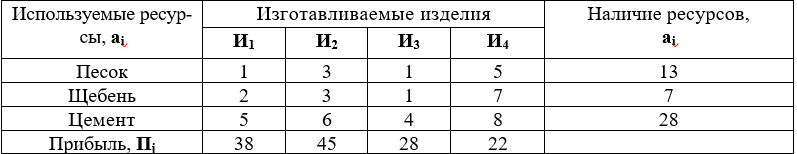
\includegraphics[scale=0.5]{1}
\newpage
\begin{center} {\bf3. Введение} \end{center}
\par
\normalsize 1.В современном мире технологие неудержимо летят вперед, с каждым годом электонно вычеслительная техника становиться мощнее, компактнее и сложнее, а людям приходиться решать все более сложные задачи. С этим людям стали помогать математические пакеты и системы компьютерной алгебры, которые во много раз сокращают время на решение сложнейших задач, с бесчисленным колличеством чисел, сейчас такие программы доступны каждому, хоть и не все они бесплатные.
\newpage
\begin{center}{\bf4.Исследование функции}
\end{center}
\par\normalsize1. Даны функции:
\\$f(x)=\sqrt{3}sin(x)+cos(x)$\\ 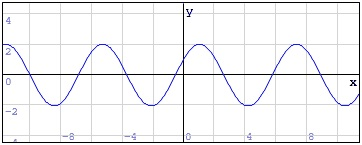
\includegraphics{f(x)}
\\$g(x)=cos(2x+\frac{\pi}{3})-1$\\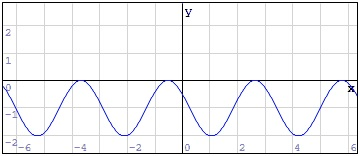
\includegraphics{g(x)}
\\a)Решить уравнение f(x)=g(x).
\\б)Исследовать функцию h(x)=f(x)-g(x) на промежутке $[0;\frac{5\pi}{6}]$\\
{\bfРешение уравнения.}
\\h(x)=f(x)-g(x)
\\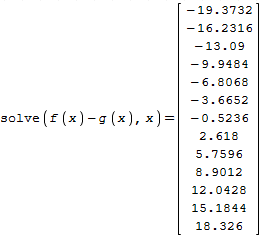
\includegraphics{11}
\newpage
\par
\normalsize
Корни функции f(x)=g(x) совпадают с корнями исследуемой функции h(x)=f(x)-g(x) и представлены выше.
\\ h(x)=f(x)-g(x)
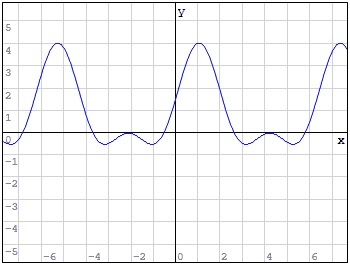
\includegraphics{h(x)=f(x)-g(x)}\\
\begin{tikzpicture}

\begin{scope}[scale=1]

\draw[thin, ->] (-7,0) -- (7,0) node[right] {$X$};
\draw[thin, ->] (0,-4) -- (0,4) node[left] {$Y$};

\draw[domain=-7:7, smooth, blue] plot ({\x},{(sqrt(3)*sin(\x r)+cos(\x r))}) node[right] {$f(x)$};
\draw[domain=-7:7, smooth, red ] plot ({\x},{cos(\x*2 r + pi/3 r)-1)}) node[right] {$g(x)$};
\draw[domain=-7:7, smooth, green] plot ({\x},{(sqrt(3)*sin(\x r)+cos(\x r))-(cos(\x*2 r + pi\3 r)-1))})node[right]{$h(x)$};
\end{scope}
\end{tikzpicture}

\newpage
\begin{tikzpicture}

\begin{scope}[scale=2]



\draw[thin, ->] (0,0) -- (3,0) node[right] {$X$};
\draw[thin, ->] (0,0) -- (0,4) node[left] {$Y$};
\draw[domain=0:2.618, smooth, green] plot ({\x},{(sqrt(3)*sin(\x r)+cos(\x r))-(cos(\x*2 r + pi/3 r)-1))})node[right];


\end{scope};

\end{tikzpicture}

Найдем корни и пересечения с осями.
\\Область определения функции задана и равна от $x=0$ до $x=\frac{5\pi}{6}$
\\Так как функция h(x)является функцией общего вида то и на области определения она также обладает общим видом если брать функцию h(x)полностью то она переодична так как повторяется при каждом изменении x на $6*\frac {5\pi}{6}$ но так как область определения составляет 1/6 от периода повтора функция не повторяется в области определения что означает у нее отсутствует периодичность
\par
\normalsize
\\1.Найдем пересечение с осью Х
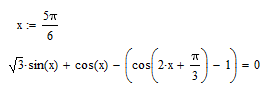
\includegraphics[scale=0.70]{3}
\\2.Найдем пересечение с осью Y
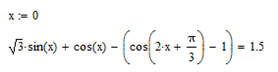
\includegraphics[scale=0.70]{4}
\newpage
\\3.Найдем экстремум в пределах области определения
\\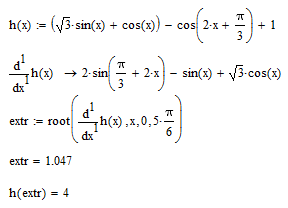
\includegraphics[scale=0.8]{5}
\\4.Функция не имеет разрывов 
\\5.Так как функция являеться изначально синусоидальной асимптот не имеет
\\6.Имеет выпуклость (0;2618)
\\7.Точек перегибов не имеет

\newpage
\begin{center}{\bf5. Исследование кубического сплайна.}\end{center}
\par
\normalsize Найти коэффициенты кубического сплайна, интерполирующего данные, представленные в векторах:\\
$V_{x}=[0,1,1.8,2.5,4]$
$V_{y}=[4,3.9,4.575,4.667,5.833]$\\
Построить на графике функции f(x), полученные после нахождения коэффицентов кубического сплайна. 
\\Оценить погрешность интерполяции в точке х=2.8 Вычислить значение функции в точке х=1.8
\\Представить графическое изображение результатов интерполяции исходных данных. 
\newpage
\begin{center}{\bf Нахождение коэффициентов кубического сплайна.}\\\end{center}
\par
\normalsize
Найдем уравнение сплайна проходящего через пять точек $(x_{1}, y_{1}),\\ 
(x_{2}, y_{2}), (x_{3}, y_{3}) и (x_{4}, y_{4})$. Для того чтобы потенциальная энергия изогнутой
металлической линейки(сплайна) принимала минимальное значение,
производная четвертого порядка должна быть равна нулю, значит мы
можем представить сплайн полиномом третьей степени на каждом отрезке
$[x_i, x_{i+1}]$
\\$$F_i(x) = A_{i0} + A_{i1}x + A_{i2}x^2 + A_{i3}x^3, где x \in [x_i, x_{i+1}]$$
\par
\normalsize По такому же принципу составляем 8 уравнений, по два на каждый участок кривой.
\begin{center}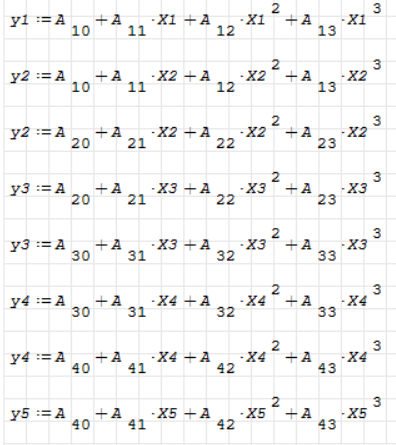
\includegraphics[scale=0.6]{12}\end{center}
\par
\newpage
\normalsize
Для того, чтобы не было излома сплайна добавляем три уравнения с производными первого порядка, по одному на каждое соединение.
\begin{center}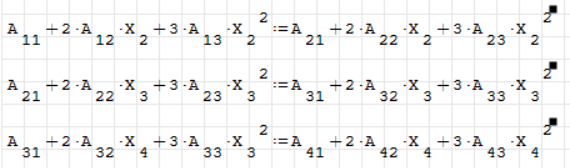
\includegraphics[scale=0.6]{13}\end{center}
\par
\normalsize
Для получения одинакового изгиба с каждой стороны стыков добавляем три уравнения с производными второго порядка.
\begin{center} 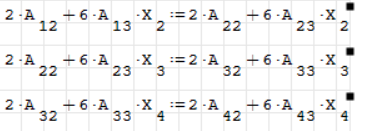
\includegraphics[scale=0.6]{14}\end{center}
\par
\normalsize
Добавим уровнения отвечающие за положение концов сплайна, в нашем случае они оставлены свободно.
\begin{center}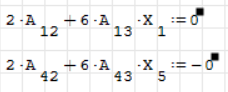
\includegraphics[scale=0.6]{15}\end{center}
\newpage
\par
\normalsize
Таким образом были найдены 16 уровнений из которых можно составить матрицу размерностью 16х16. С ее помощью, решая матричное уровнение, находим коофиценты кубического сплайна.
\begin{center}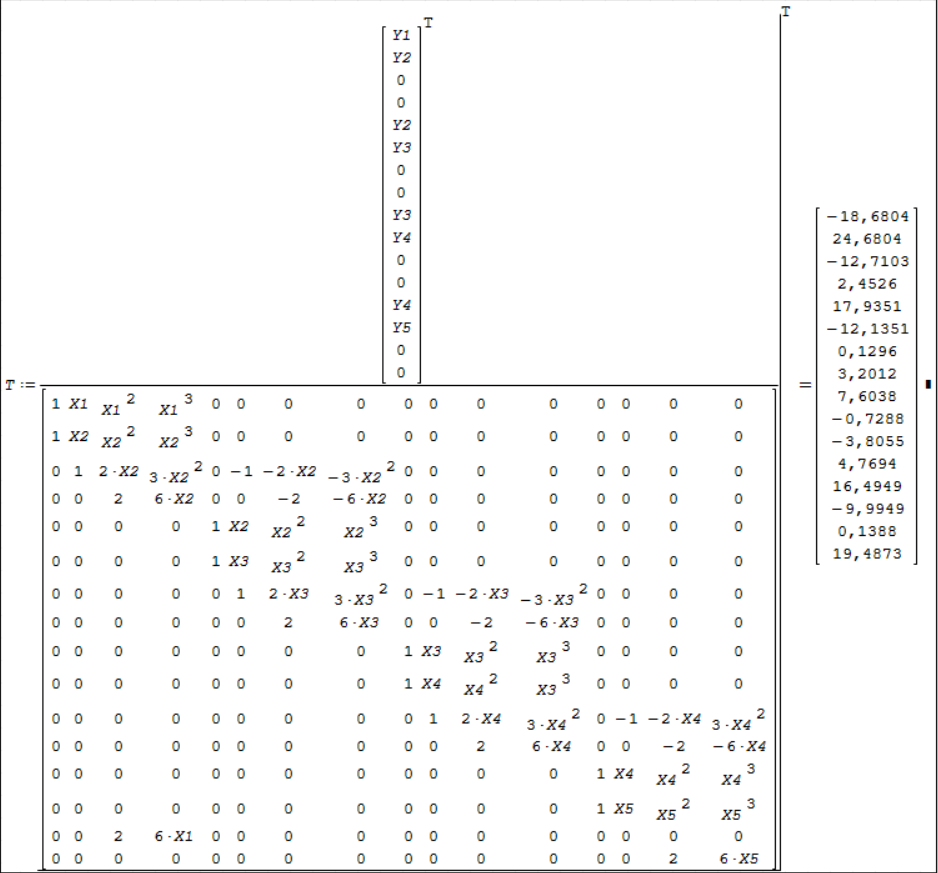
\includegraphics[scale=0.6]{6}\end{center}

\par
\normalsize
Получаем окончательное уравнение сплайна.
\begin{center}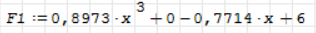
\includegraphics[scale=1]{7}\end{center}
\begin{center}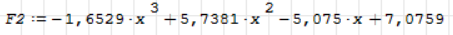
\includegraphics[scale=1]{8}\end{center}
\begin{center}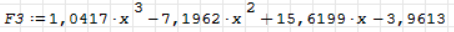
\includegraphics[scale=1]{9}\end{center}
\begin{center}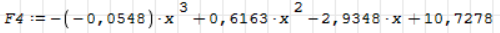
\includegraphics[scale=1]{10}\end{center}
\newpage
\begin{center}{\bf построение кубического сплайна.}\\\end{center}

\begin{tikzpicture}

\begin{scope}[scale=2]


\draw[thin, ->] (0,0) -- (7,0) node[right] {$X$};
\draw[thin, ->] (0,0) -- (0,7) node[left] {$Y$};

\foreach \x\xtext in {0,1,2,3,4} 
\draw (\x,0.1) -- (\x,-0.1) node[below] {$\xtext$};
\foreach \y\ytext in {1,2,3,4,5,6} 
\draw (0.1,\y) -- (-0.1,\y) node[left] {$\ytext$};


\draw[domain=0:0.75, smooth, blue] plot
({\x},{0.8973*(\x^3)-(0.7714*(\x))+6});

\draw[domain=0.75:1.6, smooth, red] plot ({\x},{(-1.6529*(\x^3)+(5.7381*(\x^2))-(5.075*(\x))+7.0759}); 

\draw[domain=1.6:2.375, smooth,green] plot ({\x},{(1.0417*(\x^3)-(7.1962*(\x^2))+15.6199*(\x))-3.9613});

\draw[domain=2.375:3.75, smooth, violet] plot ({\x},{(-0.0548*(\x^3)+(0.6163*(\x^2))-(2.9348*(\x))+10.7278});'
\draw(0,6) circle (0.7pt);
\draw (0.75,5.8) circle (0.7pt);
\draw (1.6,6.875) circle (0.7pt);
\draw (2.375,6.5) circle (0.7pt);
\draw (3.75,5.5) circle (0.7pt);

\draw[thin,dashed] (0.75,5.8) -- (0.75,0);

\draw[thin,dashed] (1.6,6.875)  -- (1.6,0) ;

\draw[thin,dashed]  (2.375,6.5) --  (2.375,0);

\draw[thin,dashed] (3.75,5.5) -- (3.75,0);
\end{scope};
\end{tikzpicture}
\\Воспользовавшись функцией interp в пакете Mathcad я нашел значение сплайна в точке $x=2.4$ в данной точке функция равна 6.5
\newpage
\begin{center}

{\bf Оценка погрешности интерполяции эрмитовыми
кубическими сплайнами}

\end{center}
Для того что бы найти погрешность данным способом нам нужно получить четвертую производную функции и подставить ее в формулу:
\\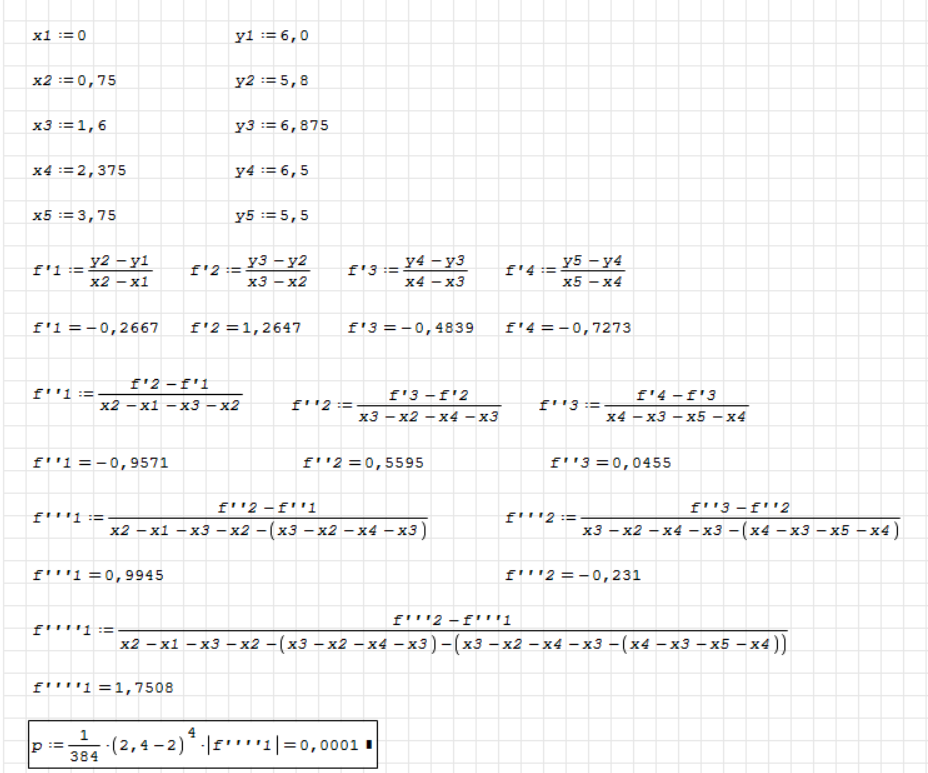
\includegraphics[scale=0.9]{2.PNG}
\\Подставив производную в формулу мы видим что погрешность в точке Х=2.4 не превышает 0.0001
\newpage 
\par 
\normalsize 
{\bf6. Задача оптимального распределения неоднородных ресурсов.}\\ 
Требуется решить следующую задачу оптимального распределения неоднородных ресурсов. Пусть в распоряжении завода железобетонных изделий (ЖБИ) имеется m видов сырья (песок, щебень, цемент) в объемах $ a_i$ .Требуется произвести продукцию n видов. Дана технологическая норма $c_ij$ требления отдельного i-го вида сырья для изготовления единицы продукции каждого j-го вида. Известна прибыль $П_j$ получаема от выпуска единицы продукции j-го вида. Требуется определить, какую продукцию и в каком количестве должен производить завод ЖБИ, чтобы получить максимальную прибыль.\\ 
Исходные данные:\\ 

\begin{center} 
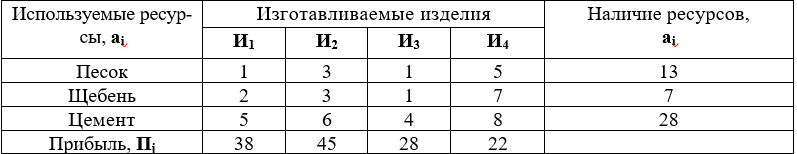
\includegraphics[scale=1]{1} 
\end{center} 
Так как данная задача является целочисленной задачей линейного программирования, стандартная функция мат. пакета «SciLab» для решения задач линейного программирования karmarkar не даст верного решения, так как не учитывает целочисленное ограничение 
Для решения задачи воспользуемся пакетом lpsolve: 

[x,f] = $lp\_solve(F,a,b,e,vlb,[],xint), где:$ 

a – матрица значений технологической норм 

B – вектор ограничений на объем используемого сырья 

F – вектор значений целевой функции - прибыли 

e – вектор, определяющий оператор отношения для ограничений $(\leq = \geq)$ 

vlb – вектор, задающий нижнюю границу переменных 

xint – вектор, задающий целочисленное ограничение на переменные 


a = [1,3,1,5;2,3,1,7;5,6,4,8]; 

B = [13,7,28]’; 

F = [38,45,28,22]; 

e = [-1,-1,-1]; 

vlb = [1,1,1]; 

xint = [0,1,2,3]; 

[x,f] =lp\_solve(F,a,B,e,vlb,[],xint) 

x = [2;0;0;0] 

f = 68. 

Таким образом, искомым целочисленным решением доставляющим максимум целевой функции является вектор [2;0;0;0], а значением целевой функции, отвечающему этому вектору = 68. Следовательно что бы получить максимальную прибыль равной 68 условных единиц, заводу нужно произвести изделие И$_1$ в размере трех штук.

\newpage
\begin{center} {\bf7. Вывод} \end{center}
Мною были изучены возможности определенного списка математических программ, а так же получено понимание выбора эффективного решения определенной задачи. Были решены задачи по исследованию функции, построению сплайна и нахождению его погрешности, а так же по решению задачи с целочисленным програмированием.



\newpage
{\bf8. Список литературы}
\\1.Ю.С. Завьялов. Методы сплайн-функций. М.Наука, 1980.
\\2.Introduction in SciLab
\\3.http://www.nsc.ru/win/docs/TeX/Tobias/lshort2e.html
\\4.http://lpsolve.sourceforge.net/5.1/Scilab.htm
\\5.smath studio user’s manual



\end{document}





